\documentclass[12pt, oneside, a4paper]{article}
\usepackage{ifpdf}
\usepackage[colorlinks,bookmarksopen,linkcolor=black,pdfauthor={Sharad,Prabhakar,Vikram},urlcolor=blue]{hyperref}
\usepackage{graphicx}

\begin{document}
\begin{center}
\pagenumbering{roman}
\thispagestyle{empty}
\textbf{Sri Jayachamarajendra College of Engineering, Mysore - 570006 \\}
\textbf{\\Department of Computer Science and Engineering}
\vspace{.5in}

\begin{figure}[htb]
\begin{center}
\ifpdf

\includegraphics[scale=0.50]{./logo.png}
\else
\fi
\end{center}
\end{figure}
\vspace{.5in}
Software Design Specification Document for\\
\textbf{\underline{Telephone Bill Generation Software for Telecom District}} \\
\vspace{.25in}
Dec 2009

\vspace{1in}

THE TEAM \\

\vspace{.1in}
\begin{tabular}{|c|c|c|}
\hline
%% row 1
 Name
& Roll Number  
& USN
\\\hline
%% row 2
Vikram TV 
& 59
& 4JC07CS120
\\\hline
%% row 3
Prabhakar Gouda
& 35
& 4JC07CS070
\\\hline
%% row 4
Sharad D
& 03
& 4JC06CS089
\\\hline
\end{tabular}
\\ **5th Semester 'B' Section
\end{center}
\newpage
\thispagestyle{empty}
\tableofcontents
\newpage
\pagenumbering{arabic}

\section{Introduction}
\subsection{Purpose}
	This design document provides the design for implementing the \textbf{Telephone Bill Generation for Telecom District}. This includes the architectural features of the system and details of each schema used in the design.
	
\subsection{Scope}
	To design efficient and user friendly online billing system for telecom district.  The dominant design methodology used would be \emph{function oriented} with a \emph{visual interface} for the database.\\
	The billing records that are updated in the database are retrieved and the processing of the retrieved database is done mainly by the Visual interface.  After the processing is done, it is suitably outputted (as per user requirements) by a front-end.\\
All the customers access the database using the form based approach.\\
The administrator can access database either by forms or directly using database management systems like MySQL, PHPMyAdmin.

\subsection{Glossary}
\begin{tabular}{ll}
TelBill & Telephone Bill generation System\\
Users & Administrator, Authorized Staff of Telecommunication Company, Customers\\
CustomerID &  Unique key for identifying the customer in the database.\\
BillNo & Unique key in identifying each bill.\\
ReceiptNo & Unique key for identifying each payment of the bill.\\
logs & Call Logs, it can be received or dialed calls.\\
\end{tabular}

\subsection{References}
Software Engineering by Ian Sommerville, 6th Edition\\
BSNL Telephone Bill\\
\href{http://data.bsnl.in}{BSNL Portal} for Usage Check\\
\href{http://standards.ieee.org/reading/ieee/std_public/new_desc/se/1016-1998.html}{IEEE Documentation Format} for SDS

\newpage

\section{Software Lifecycle}
The TelBill software lifecycle includes the following phases:
\begin{itemize}
\item Requirements
\item Design
\item Implementation
\item Test
\item Installation
\item Operation and Maintenance
\end{itemize}

\begin{figure}[htb]
\begin{center}
\ifpdf
	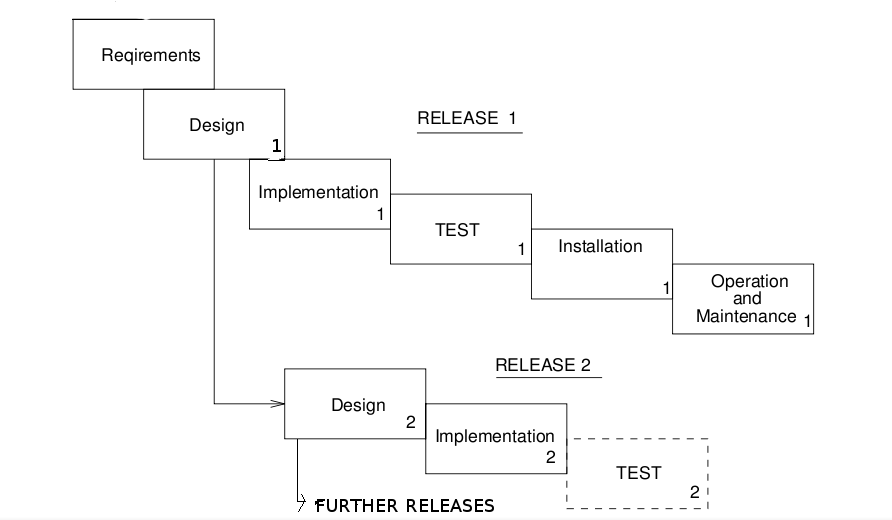
\includegraphics[scale=0.50]{./lifecycle.png}
\else
\fi
\caption{Life Cycle of TelBill}
\label{Life Cycle}
\end{center}
\end{figure}
The software is done in multiple releases making use of the \emph{spiral development model}.  Each release is updated with new functionalities and features. Development activities starts from the design phase of previously released versions.  The act of releasing depends on user suggestions and also on technology updations.
\newpage

\section{Architectural Design}
The architectural design of the TelBill consists of identifying the various users and their representation in the database.  Maintaining a centralised database for all the users simplifies the task of querying the database.  The modules are created for database storage and are linked together by the foreign keys.  The task of bill generation also includes the handling of customer information, phone numbers, meter readings, tariffs, call logs and finally the bill details and payment details.  A login database also needs to be specified for security.

\subsection{Overall System Organisation being Shared Data Repository}
The shared centralised data in the database can be accessed by
\begin{itemize}
\item Administrator
\item Clerks
\item Technicians
\item Customers
\item Application Programs
\end{itemize}

Application programs that automate the process running in the database.


A centralised database is maintained to store the details of the telephone connections that are provided.  It also includes the customer details, call logs, meter logs, bill amounts and payment details.  The database access by the above users is as shown in the diagram.
% central repository diagram
\begin{figure}[htb]
\begin{center}
\ifpdf
	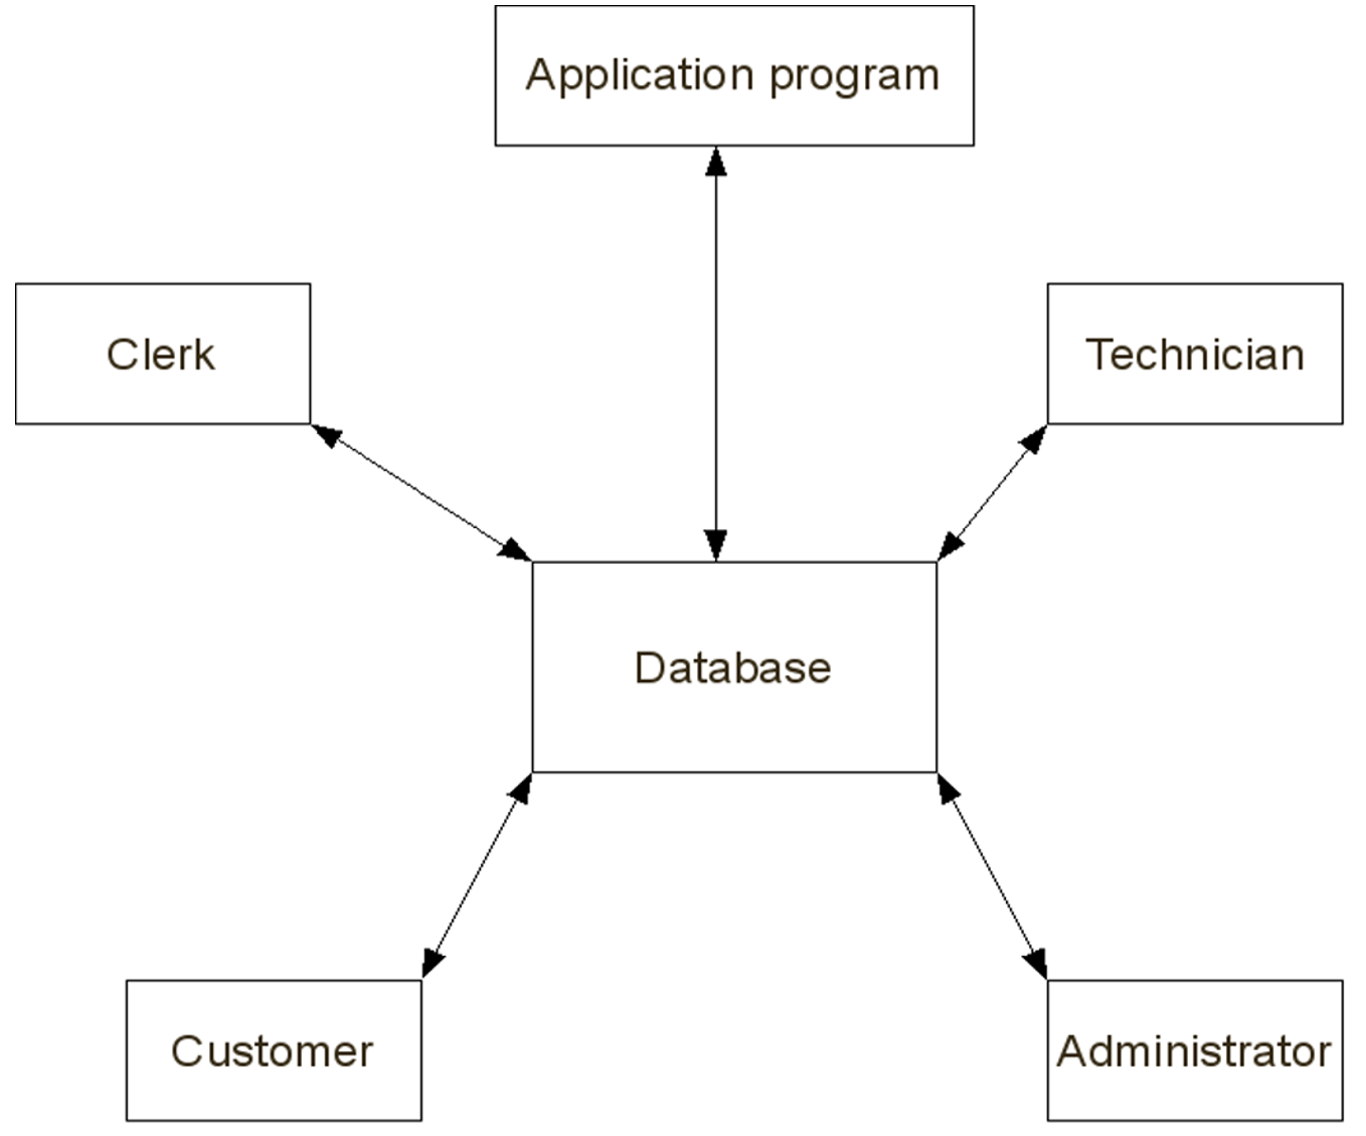
\includegraphics[scale=0.20]{./central.png}
\else
\fi
\caption{Shared Data Repository}
\label{fig: Central Repository}
\end{center}
\end{figure}
\newpage 
\subsection{Creation of Modules}
A Unique ID is used to identify a customer in the entire database.  Also bills and payment receipts are also identified by Unique Bill Number and Unique Payment Number.\\

The following nine modules are identified for the implementation of the TelBill:\\\\
\begin{tabular}{ll}
Customer & Maintains the details of the customer like name and customer ID.\\\\
Login & Maintains the login details of the user\\\\
Address & Maintains the complete address of the customer.\\\\
Tariff & Maintains the plan opted by the customer.  Bill is generated as per the tariff.\\\\
\end{tabular}
\begin{tabular}{ll}
Phone Number & Maintains the phone numbers for each customer.\\\\
Call Log & Maintains the timestamp of the dialled and received calls.\\\\
Meter Reading & Maintains the monthly start and end meter readings for each customer.\\\\
Bill & Maintains the details of the generated bill like call charges, taxes and the \\ & final bill amount.\\\\
Payment & Maintains the timestamps of bill payments.\\\\
\end{tabular}

% modules or tables diagram
\begin{figure}[htb]
\begin{center}
\ifpdf
	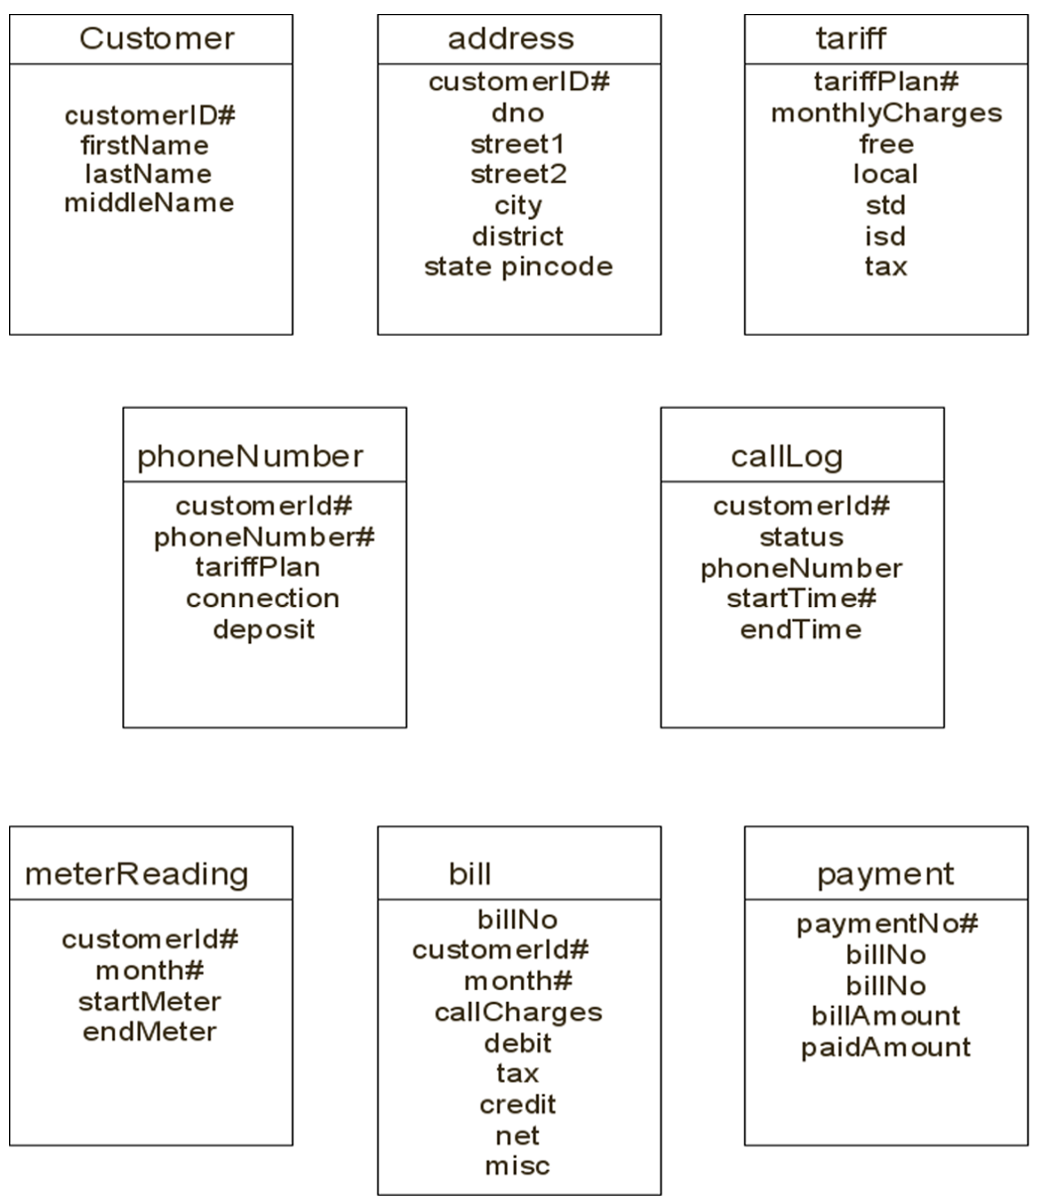
\includegraphics[scale=0.30]{./module.png}
\else
\fi
\caption{Only Modules No Connections}
\label{fig: Modules}
\end{center}
\end{figure}

\subsection{Cohesion of Modules}
The modules are interconnected to allow interfacing among them.  They are binded by refering to \emph{foreign keys}.\\
The Entity - Relationship Model specifies the key constraints and the relation between tables.\\\\\\

\begin{figure}[htb]
\begin{center}
\ifpdf
	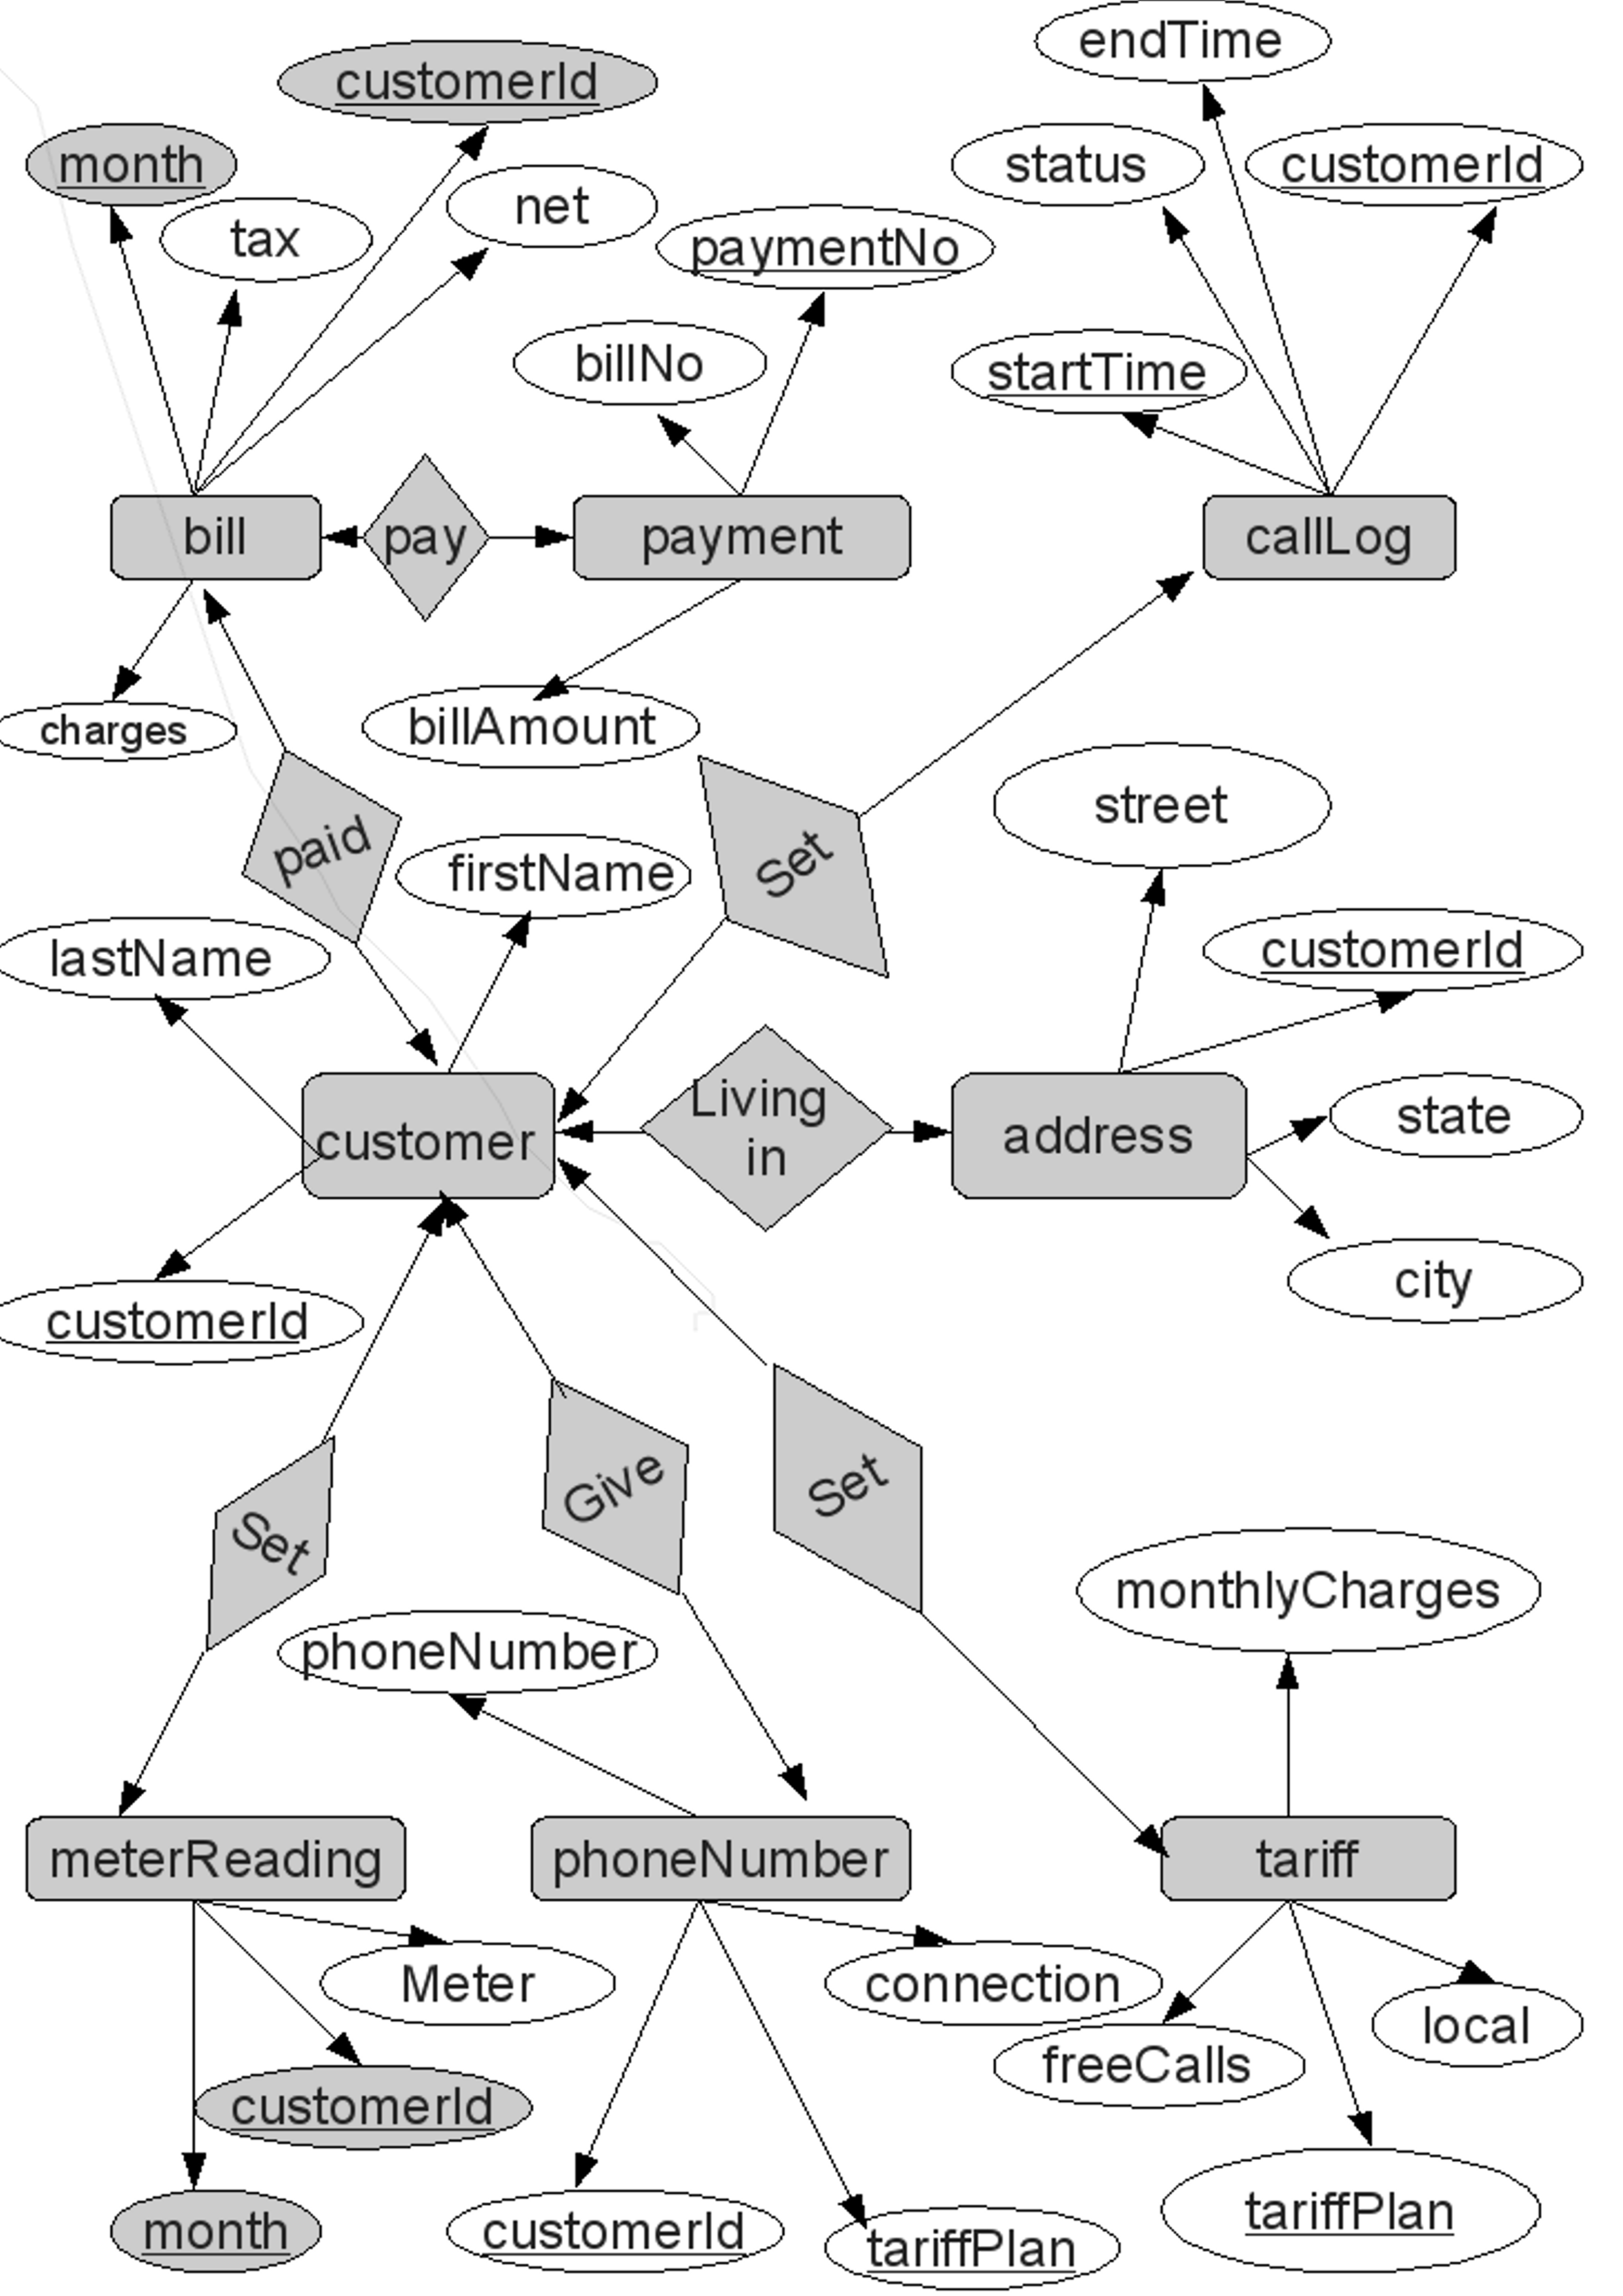
\includegraphics[scale=0.40]{./er1.png}
\else
%	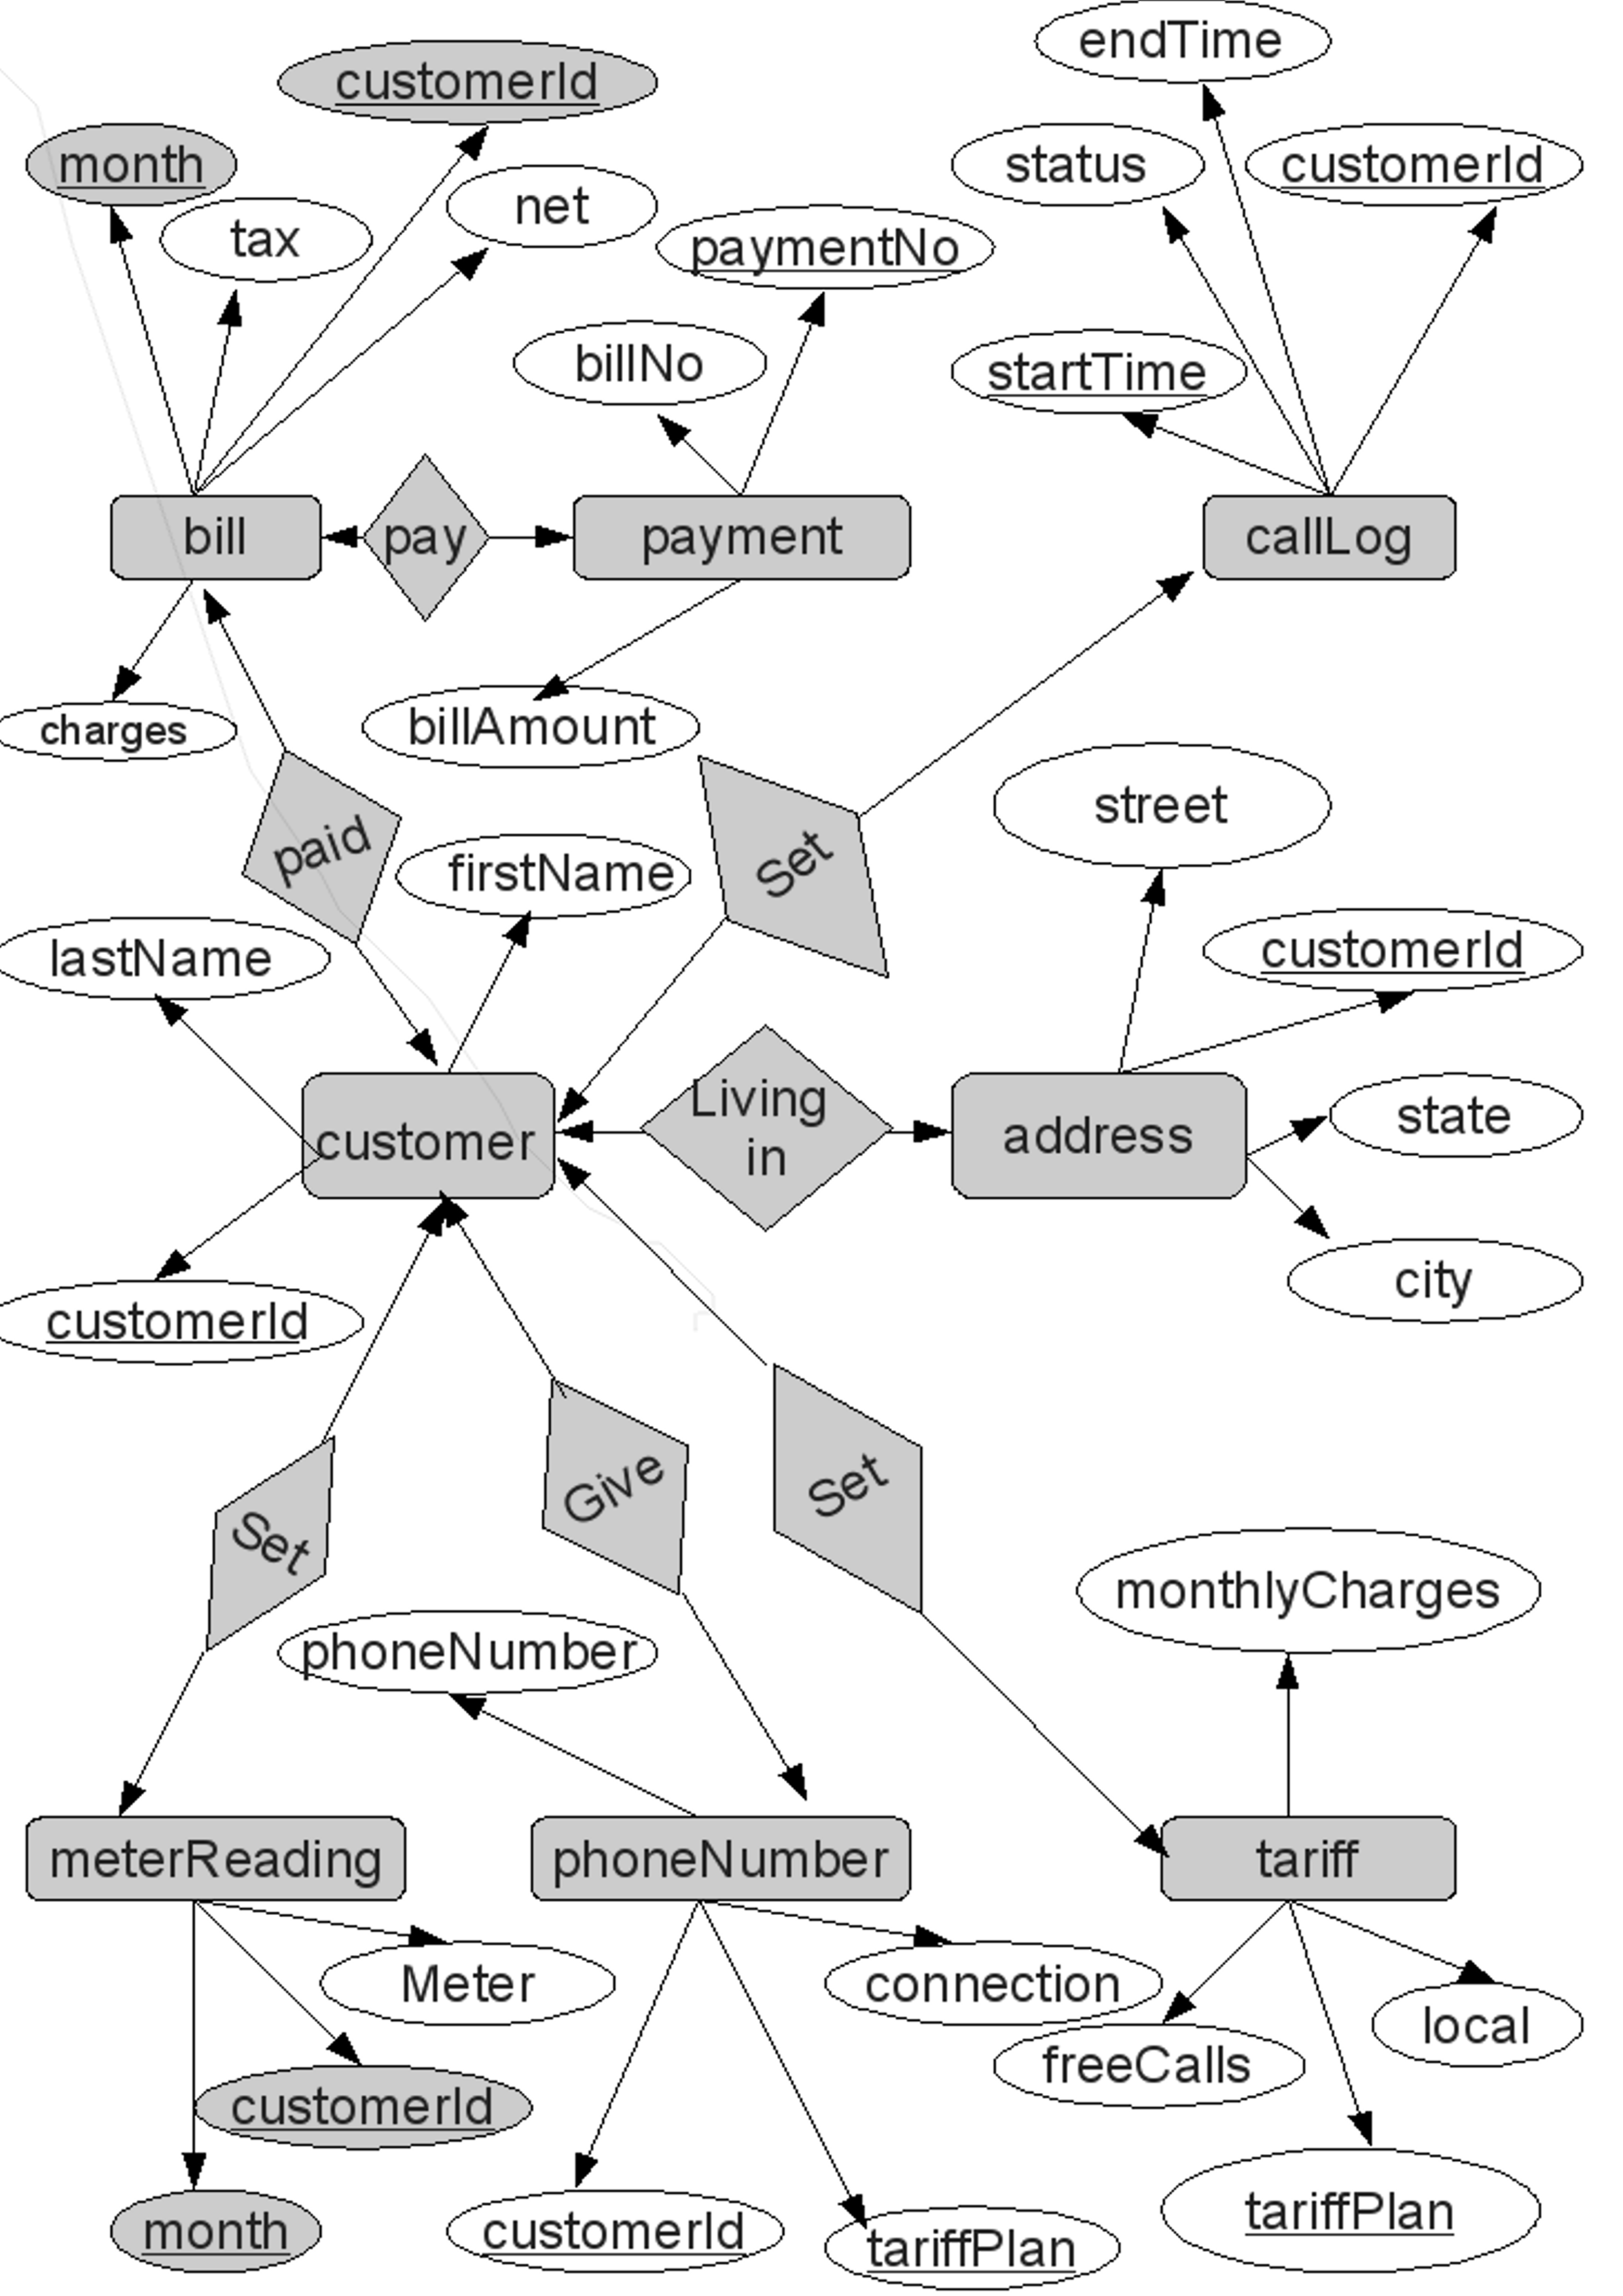
\includegraphics[scale=0.50]{./er1.png}
\fi
\caption{ER Model used in the design}
\label{fig: ER Model}
\end{center}
\end{figure}
\newpage 
The diagram describes the foreign key referenciations.\\\\\\
\begin{figure}[htb]
\begin{center}
\ifpdf
	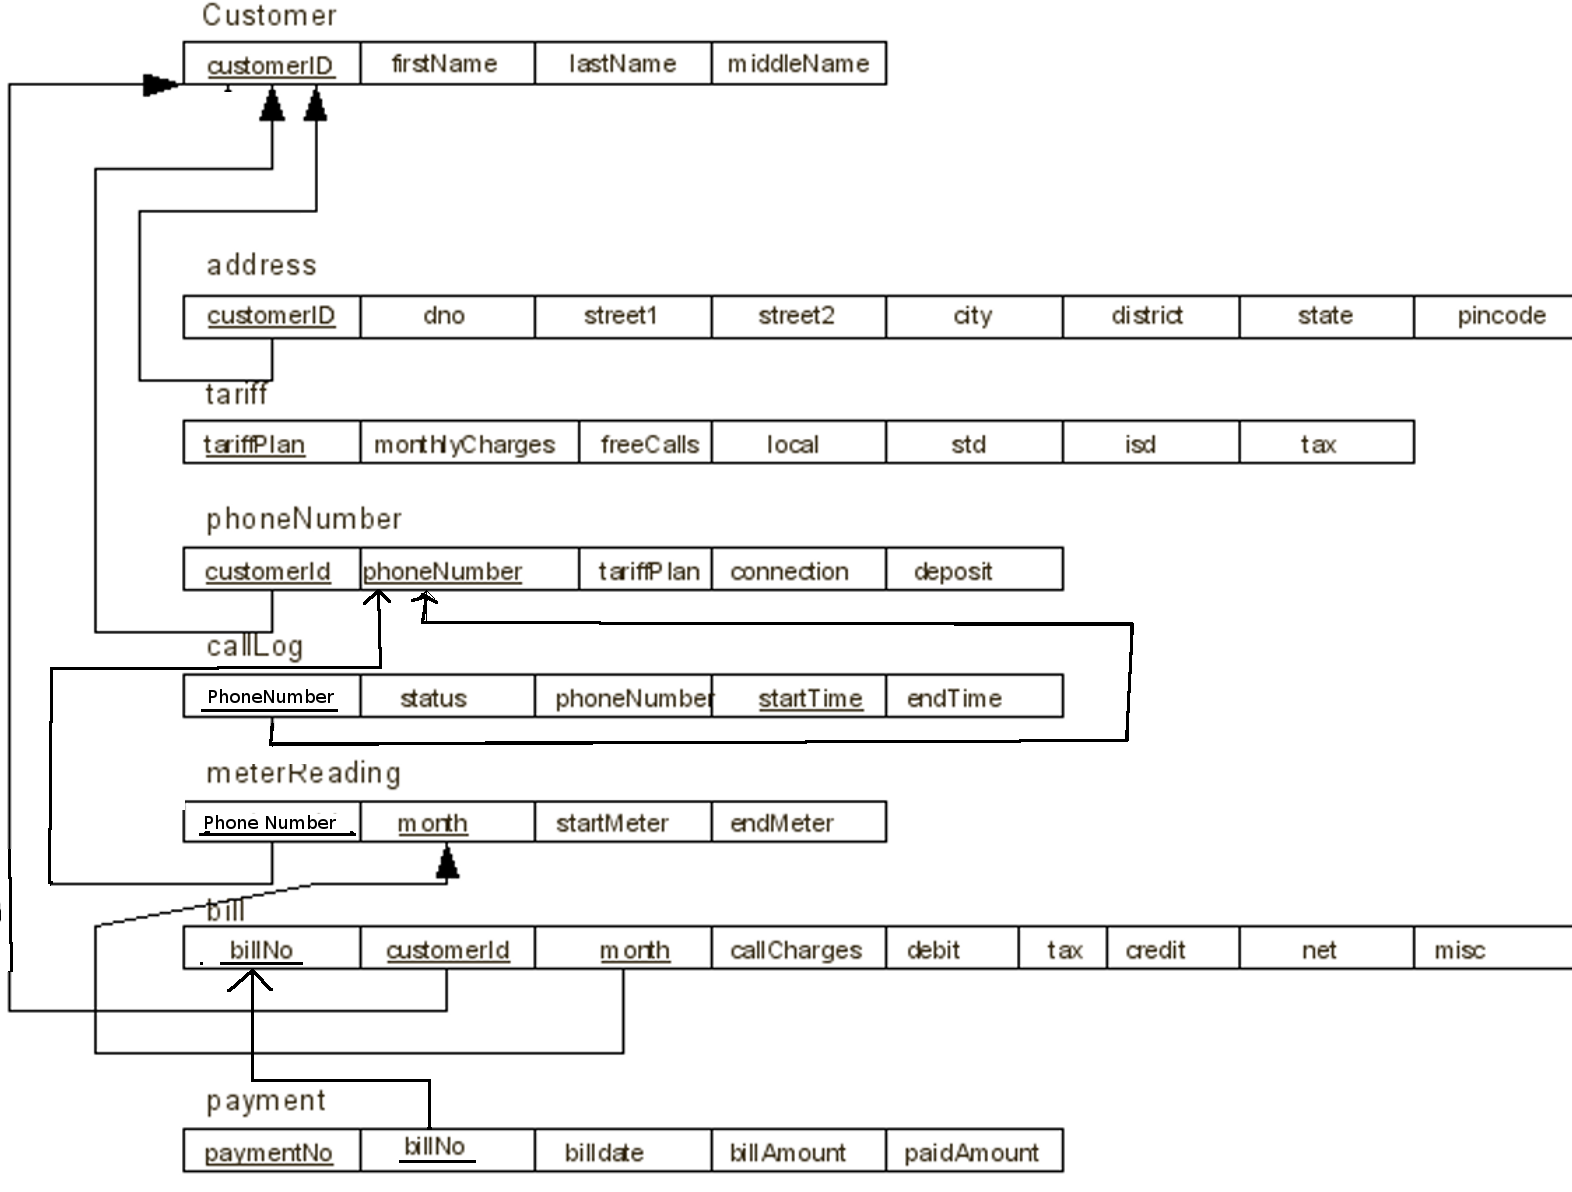
\includegraphics[scale=0.30]{./connections.png}
\else
\fi
\caption{Connecting Modules}
\label{fig: Connecting Modules}
\end{center}
\end{figure}
\newpage

\section{Detailed Design}
This section consists of detailed design of the modules, that is the datatypes used to specify the attributes used in each modules.
\subsection{Data types specifying the attributes}
The following tables specifies the attributes in each modules. It also specifies the primary keys in each modules and the foreign key referenciations for other modules.
\subsubsection{Module Customer}
\textbf{Attributes}:\\\\
\begin{tabular}{ll}
Customer ID & of integer and Auto Increment type, Unique ID for each customer\\\\
First Name & of variable string type\\\\
Middle Name & of variable string type\\\\
Last Name & of variable string type\\\\
\textbf{Primary Key } : & Customer ID\\\\
\textbf{Foreign Keys }: & NIL\\\\
\end{tabular}

\subsubsection{Module Login}
\textbf{Attributes}:\\
\begin{tabular}{ll}
Username & of variable string type, length 10\\\\
User Password & of string type, length 64 to store passwords in encrypted format\\\\
Customer ID & of integer type\\\\
\textbf{Primary Key } : & Customer ID\\\\
\textbf{Foreign Keys } : & Customer ID $\rightarrow$ Customer ID of Module Customer\\\\
\end{tabular}
\newpage
\subsubsection{Module Address}
\textbf{Attributes}:\\\\
\begin{tabular}{ll}
Customer ID & of integer type \\\\
Door Number & of variable string type\\\\
Street 1 & of variable string type\\\\
Street 2 & of variable string type\\\\
City & of variable string type\\\\
District & of variable string type\\\\
State & of variable string type\\\\
Pincode & of integer type, length 6\\\\
\textbf{Primary Key } : &  NIL (Weak entity)\\\\
\textbf{Foreign Keys }: & Customer ID $\rightarrow$ Customer ID of Module Customer\\\\
\end{tabular}

\subsubsection{Module Tariff}
\textbf{Attributes}:\\\\
\begin{tabular}{ll}
	Tariff Plan & of integer type, describes the type of plan\\\\
	Monthly Charges & of float type\\\\
	Free Calls & of integer type\\\\
	Local Call Rates &  of float type\\\\
	STD Call Rates & of float type\\\\
	ISD Call Rates & of float type\\\\
\end{tabular}\\
\begin{tabular}{ll}
	Tax Percentage & of float type\\\\	
	\textbf{Primary Keys } : & Tariff Plan\\\\
\end{tabular}

\subsubsection{Module Phone Number}
\textbf{Attributes}:\\\\
\begin{tabular}{ll}
Customer ID & of integer type\\\\
Phone Number & of integer type, Unique ID for each Phone\\\\
Tariff Plan & of integer type, describes the type of tariff\\\\
Connection Date & of date type\\\\
Deposit & of float type, describes the deposit made by the customer\\\\
\textbf{Primary Keys } : & Customer ID, Phone Number\\\\
\textbf{Foreign Keys } : & Customer ID $\rightarrow$ Customer ID of Module Customer\\\\
 & Tariff Plan $\rightarrow$ Tariff Plan of Module Tariff\\\\
\end{tabular}

\subsubsection{Module Call Logs}
\textbf{Attributes}:\\\\
\begin{tabular}{ll}
	Customer ID & of integer type\\\\
	Phone Number & of integer type\\\\
	Status & of character type, specifies Received Calls from Dialled Calls\\\\
	Start Time of Call & of  integer type\\\\
	End Time of Call & of integer type\\\\
\end{tabular}\\
\begin{tabular}{ll}

\textbf{Primary Keys } : &  Phone Number, Start Time\\\\
\textbf{Foreign Keys } : & Customer ID $\rightarrow$	 Customer ID of Module Customer\\\\	
 & Phone Number $\rightarrow$	 Phone Number of Module Phone Number\\\\	
\end{tabular}


\subsubsection{Module Meter Reading}
\textbf{Attributes}:\\\\
\begin{tabular}{ll}
	Phone Number & of integer type\\\\
	Month & of integer type, holds month and year of meter reading\\\\
	Start Meter Reading & of  integer type\\\\
	End Meter Reading & of integer type\\\\
\textbf{Primary Keys } : &  Phone Number, Month\\\\
\textbf{Foreign Keys } : & Customer ID $\rightarrow$	 Customer ID of Module Customer\\\\	
& Phone Number $\rightarrow$	 Phone Number of Module Phone Number\\\\	
\end{tabular}

\subsubsection{Module Bill}
\textbf{Attributes}:\\\\
\begin{tabular}{ll}
	Bill Number & of integer type, Unique ID for each Bill that is generated\\\\
	Customer ID  & of integer type\\\\
	Month & of integer type, holds month and year of bill generation\\\\
	Call Charges & of float type\\\\
	Debit & of float type, describes any previous debits from the customer\\\\
\end{tabular}\\
\begin{tabular}{ll}
	Tax  & of float type, describes taxation for the gross amount \\ & of bill generated\\\\
	Credit & of float type, describes any previous credits from the customer\\\\
	Net Charges & of float type, contains the net amount of the bill\\\\
	Miscellaneous Charges & of float type, describes any miscellaneous charges \\ & like installation charges, caller tune charges\\\\
\textbf{Primary Keys } : &  Customer ID, Month\\\\
\textbf{Foreign Keys } : & Customer ID $\rightarrow$	 Customer ID of Module Customer\\\\	
\end{tabular}

\subsubsection{Module Payment}
\textbf{Attributes}:\\\\
\begin{tabular}{ll}
	Payment Number &  of integer type, Unique ID for each receipts that are made\\\\
	Bill Number & of integer type\\\\
	Pay Date & of date type\\\\
	Bill Amount & of float type \\\\
	Payment Amount & of float type\\\\
\textbf{Primary Keys } : &  Payment Number\\\\
\textbf{Foreign Keys } : & Bill Number $\rightarrow$	 Bill Number of Module Bill\\\\	
\end{tabular}


\subsection{Sequence diagram for Data Collection}:
The sequence diagram shows the three layers for data flow.  They include the Front End, Processing and Database.  The following activities takes place in the sequential manner.

\begin{itemize}
\item User enters Username and Password to the front end.
\item Front end sends the username and password using the send() function to the processing layer and suspends itself.
\item The processing layer requests the database to return the password for the requested username using requestPassword() function.  After receiving the password from the database using sendPassword() function, it is checked with the password provided by the user using isValid() function.
\item If password is valid then further querying is allowed else the error is displayed by the front end.
\end{itemize}
\begin{figure}[htb]
\begin{center}
\ifpdf
	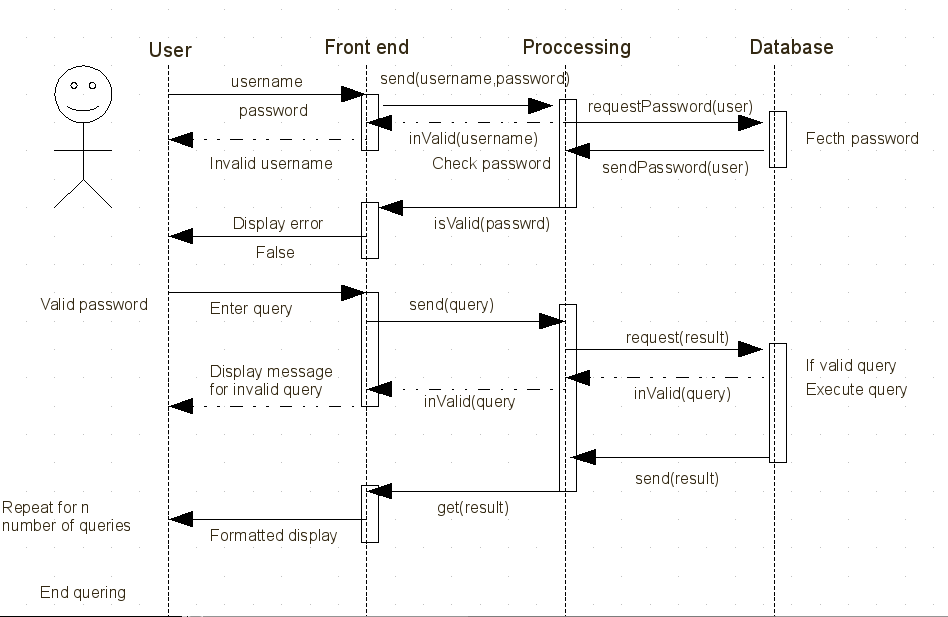
\includegraphics[scale=0.50]{./sequence.png}
\else

\fi
\caption{Data Collection Sequence Diagram}
\label{fig:Sequence Diagram}
\end{center}
\end{figure}
\begin{itemize}
\item User then queries the database using the front end like requesting the \emph{month bill, profile}.
\item These queries are also processed in the processing layer and result is requested from database using the request() function.
\item Database returns invalid query if the query is incorrect using the inValid() function that gets displayed on the screen.
\item Database executes valid query and returns result using the sendResult() function to the processing layer.
\item Processing layer format the results and sends it to the front end using the getResult() function.
\item Front end displays the result suitable and waits for further querying by the user.
\item Querying gets terminated when the user logs out.
\end{itemize}


\section{User Interface Design}
The User Interface or the \emph{frontend} supports for the user to interact with the database.  The User Interface is designed to be online so that customers can also access the database.  Hence there should be a design that supports both customers and the TelBill staff.

The following are the interfacing designs to be implemented:\\\\
\begin{itemize}
\item The passwords are encrypted (using the latest encryption algorithms - currently `message-direct-5' or md5) and stored in the database module login.userpassword and a unique username in login.username.
\item A welcome screen should greet all the users where a login prompt is also provided for users to login.

Administrator login should support for handling the entire database, other TelBill staff login should support for operations and maintenance and Customer login should support for viewing the monthly bills and their profile.
\item Administrator login should redirect to admin screen that has options to add user, customer, new connection; update users, customers, new connections; delete users, customers, new connections.  Also to perform backups and maintenance facilities.  Customize the entire environment.

The Administrator is reminded periodically to make backups.  It also reminds to \emph{clear} call logs and older bills.
\item TelBill staff login should redirect to staff screen that has options to only handle the entries that gets generated from hardwares.  Like they can view the call logs, update and view bill payments, backups, maintenance and also \emph{handle customer queries}.
\item Customer login should redirect to customer screen that has options to only view the bill and profile, make online payments.  A drop-down boxes are to be provided to select the tariff plans, phone numbers (as a single customer can have multiple phone connections) and the month to view the \emph{bill} that is generated.
\item Gross bill is not stored in database and is \emph{calculated dynamically} in the front end. 
\item A logout option is also provided for each user to safely disconnect from the database.

\item If hard copy of the bills are lost, then they can be reproduced again using the TelBill.
\end{itemize}

\section{Limitations}
\begin{itemize}
\item The current design does not support for \emph{password} retreival of any user, in case the password is lost.
\item Billing for Value Added Services or VAS provided by the service provider is not incorporated.
\end{itemize}
The above features need to be incorporated in future releases.
\section{Conclusion}
A spiral development model is specified for the design and implementation of the TelBill.  A shared data repository holds the entire database of all the interfaced modules that are accessed by all the users.  An object oriented approach was found to be suitable to implement the TelBill. Finally, all users are provided with suitable screens to interface with the database.
\end{document}
